\documentclass[a4paper, twocolumn]{article}
\usepackage[dvips]{graphicx}
\usepackage{lipsum}

\begin{document}

\lipsum[1]

\begin{figure}[!hbtp]
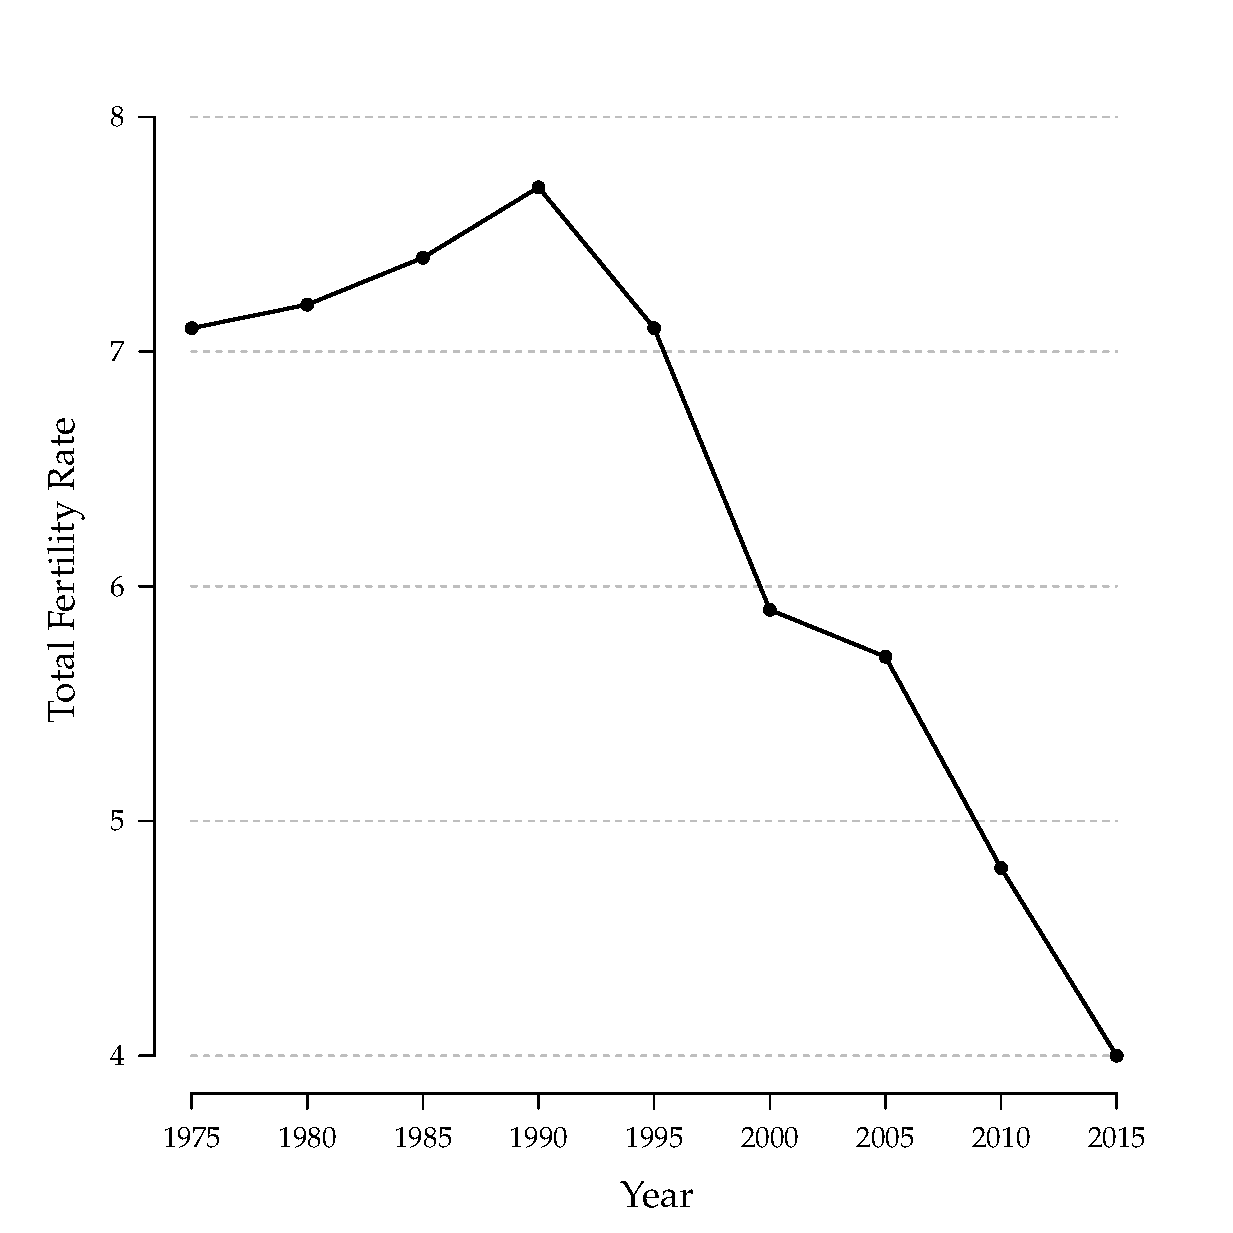
\includegraphics[width = \columnwidth]{../figures/fig1.eps}
\caption{Fig 1}
\end{figure}

\lipsum[1]

\begin{figure}[!hbtp]
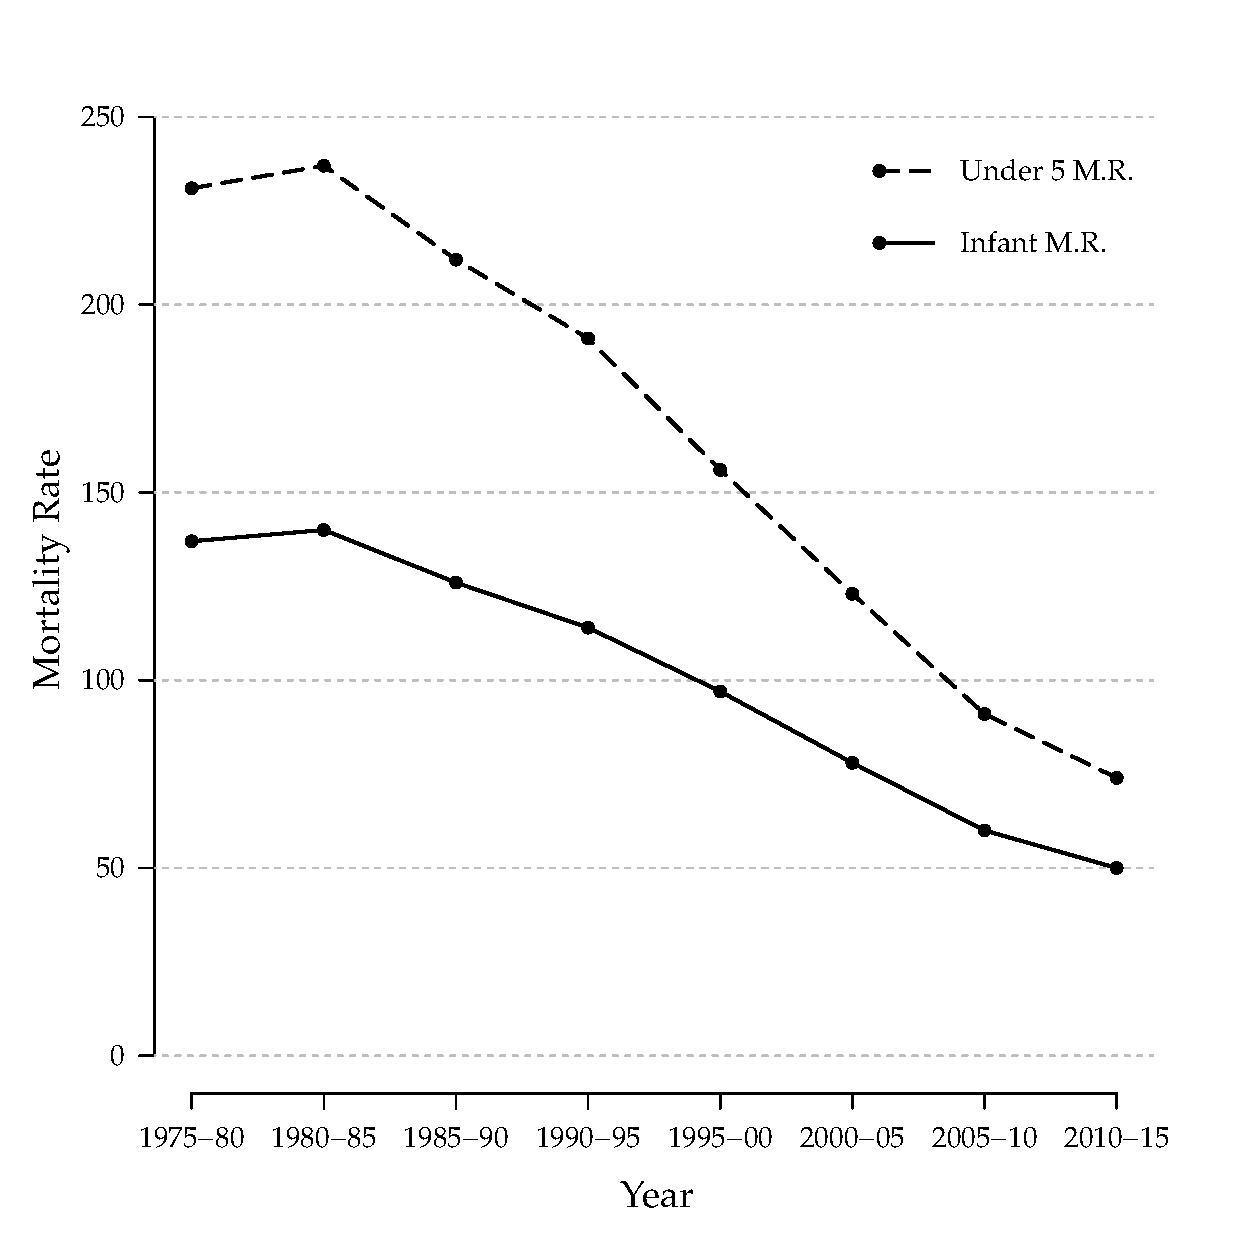
\includegraphics[width = \columnwidth]{../figures/fig2.eps}
\caption{Fig 2}
\end{figure}

\lipsum[2]

\begin{figure}[!hbtp]
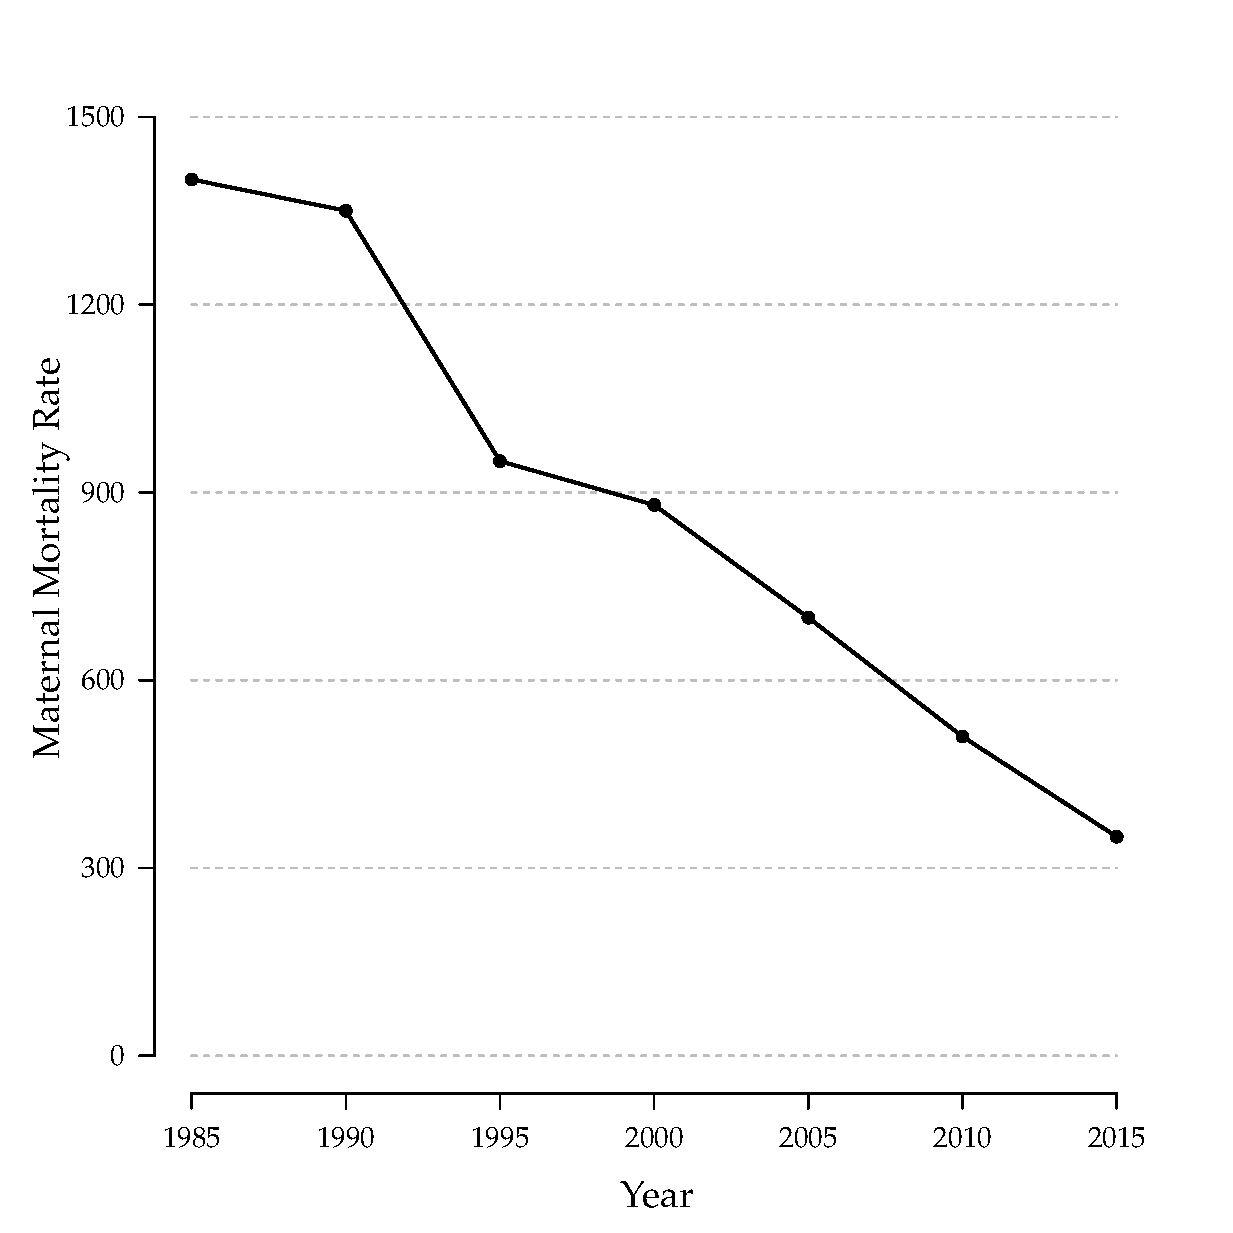
\includegraphics[width = \columnwidth]{../figures/fig3.eps}
\caption{Fig 3}
\end{figure}

\lipsum[3]

\begin{figure}[!hbtp]
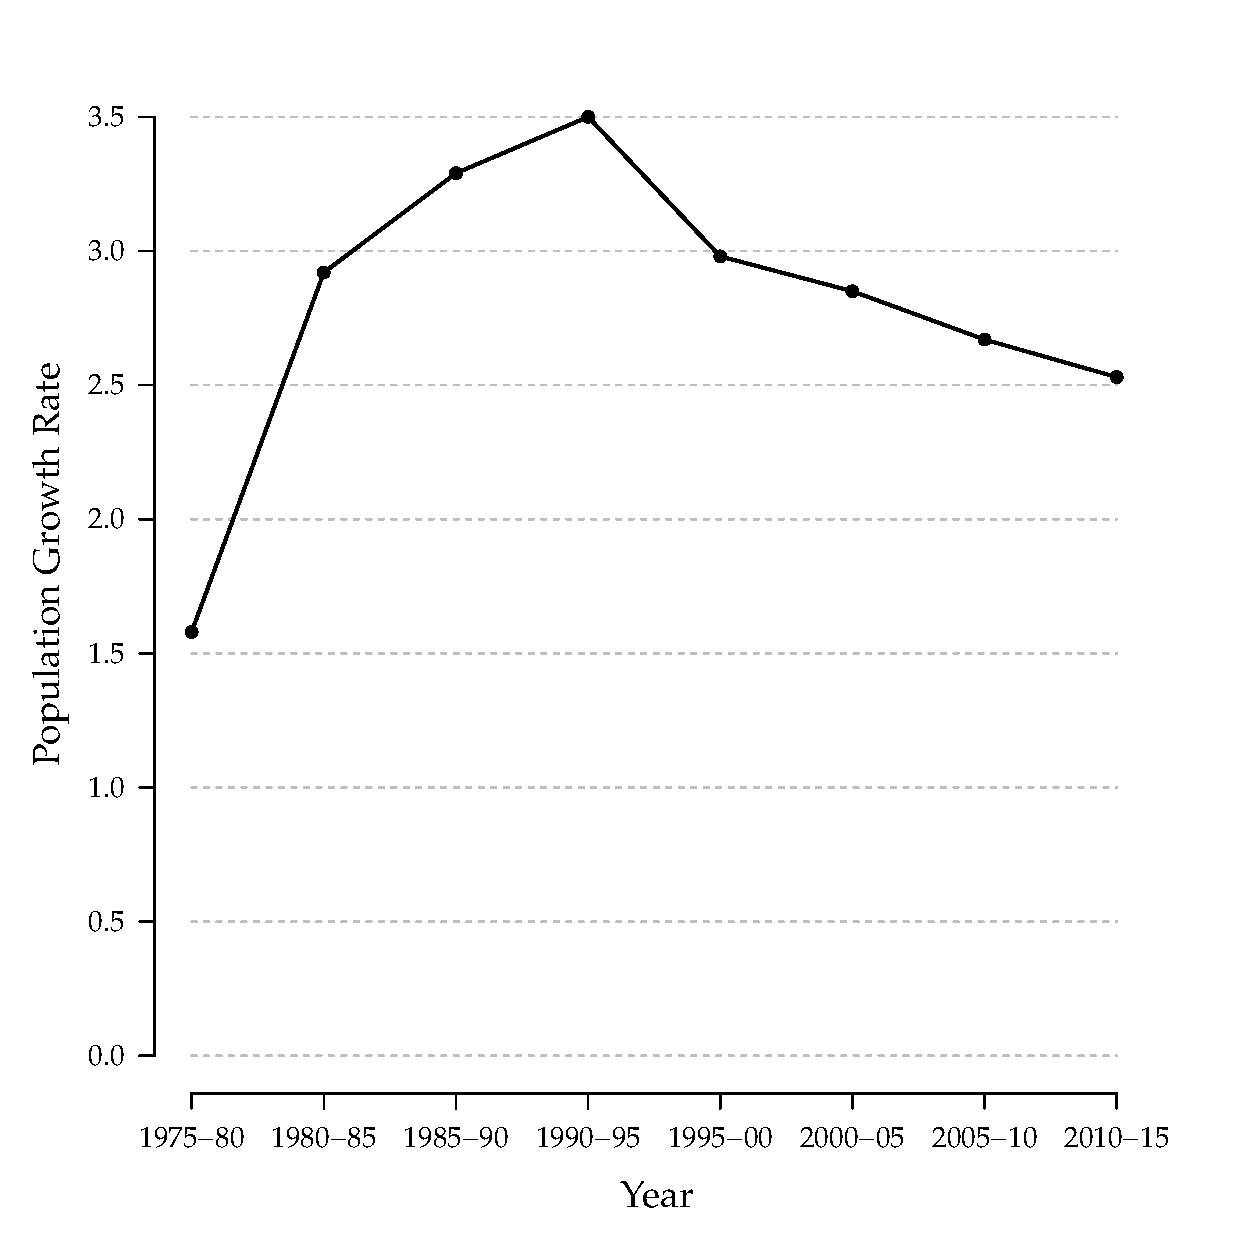
\includegraphics[width = \columnwidth]{../figures/fig4.eps}
\caption{Fig 4}
\end{figure}

\lipsum[4]


\begin{figure}[!hbtp]
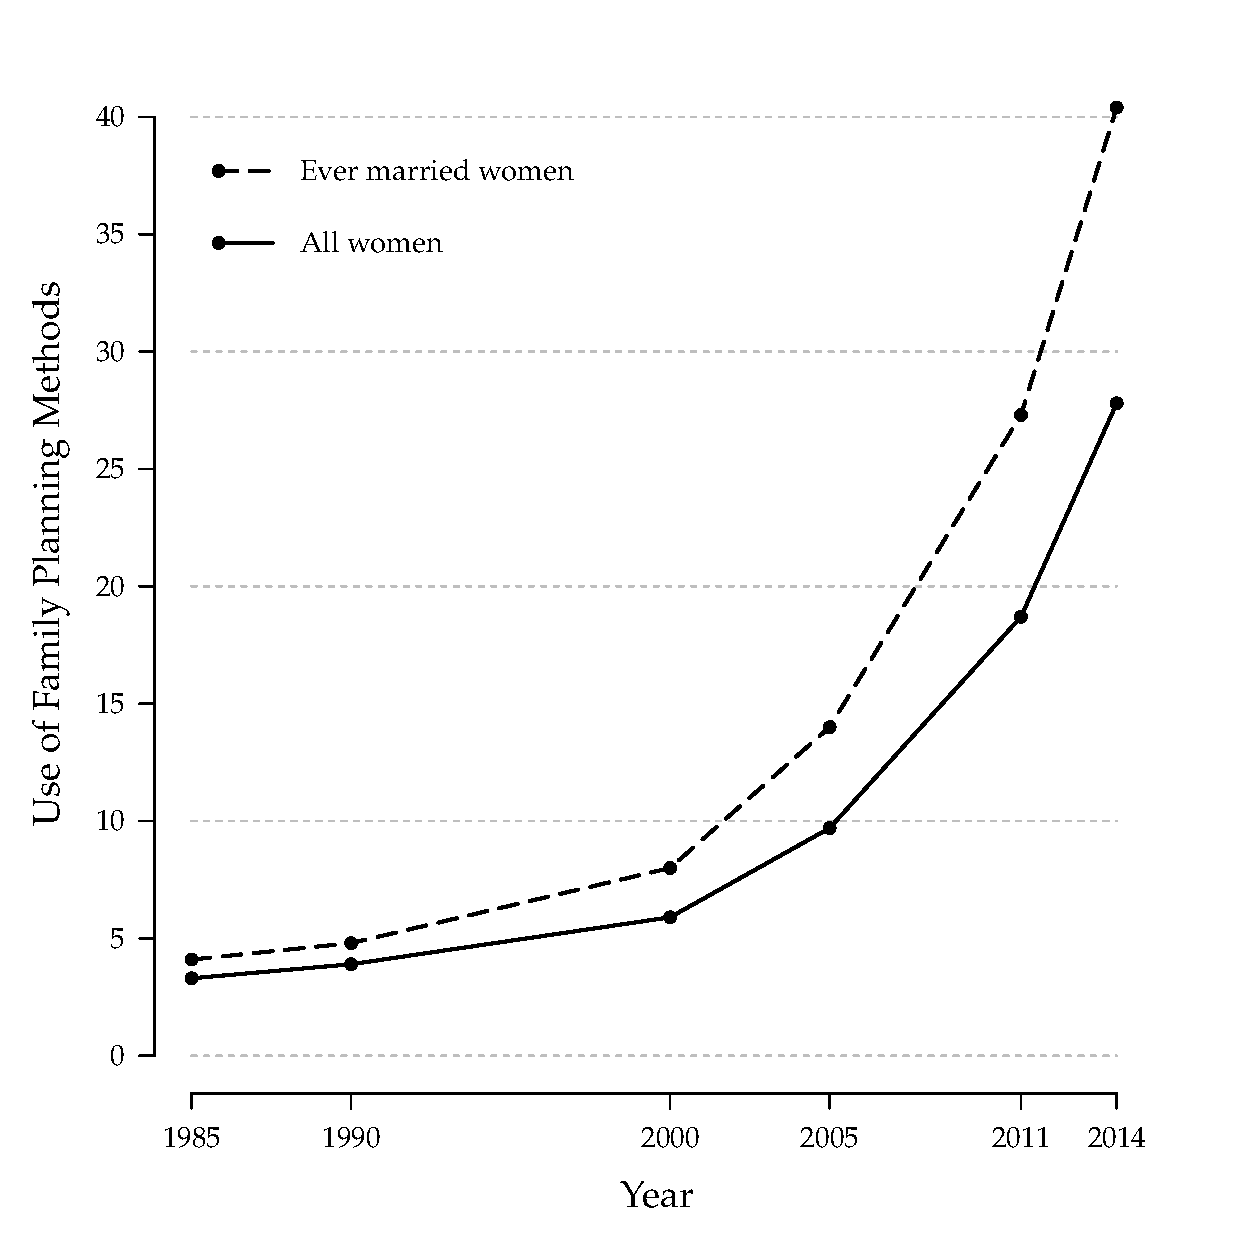
\includegraphics[width = \columnwidth]{../figures/fig5.eps}
\caption{Fig 5}
\end{figure}

\lipsum[1]

\begin{figure}[!hbtp]
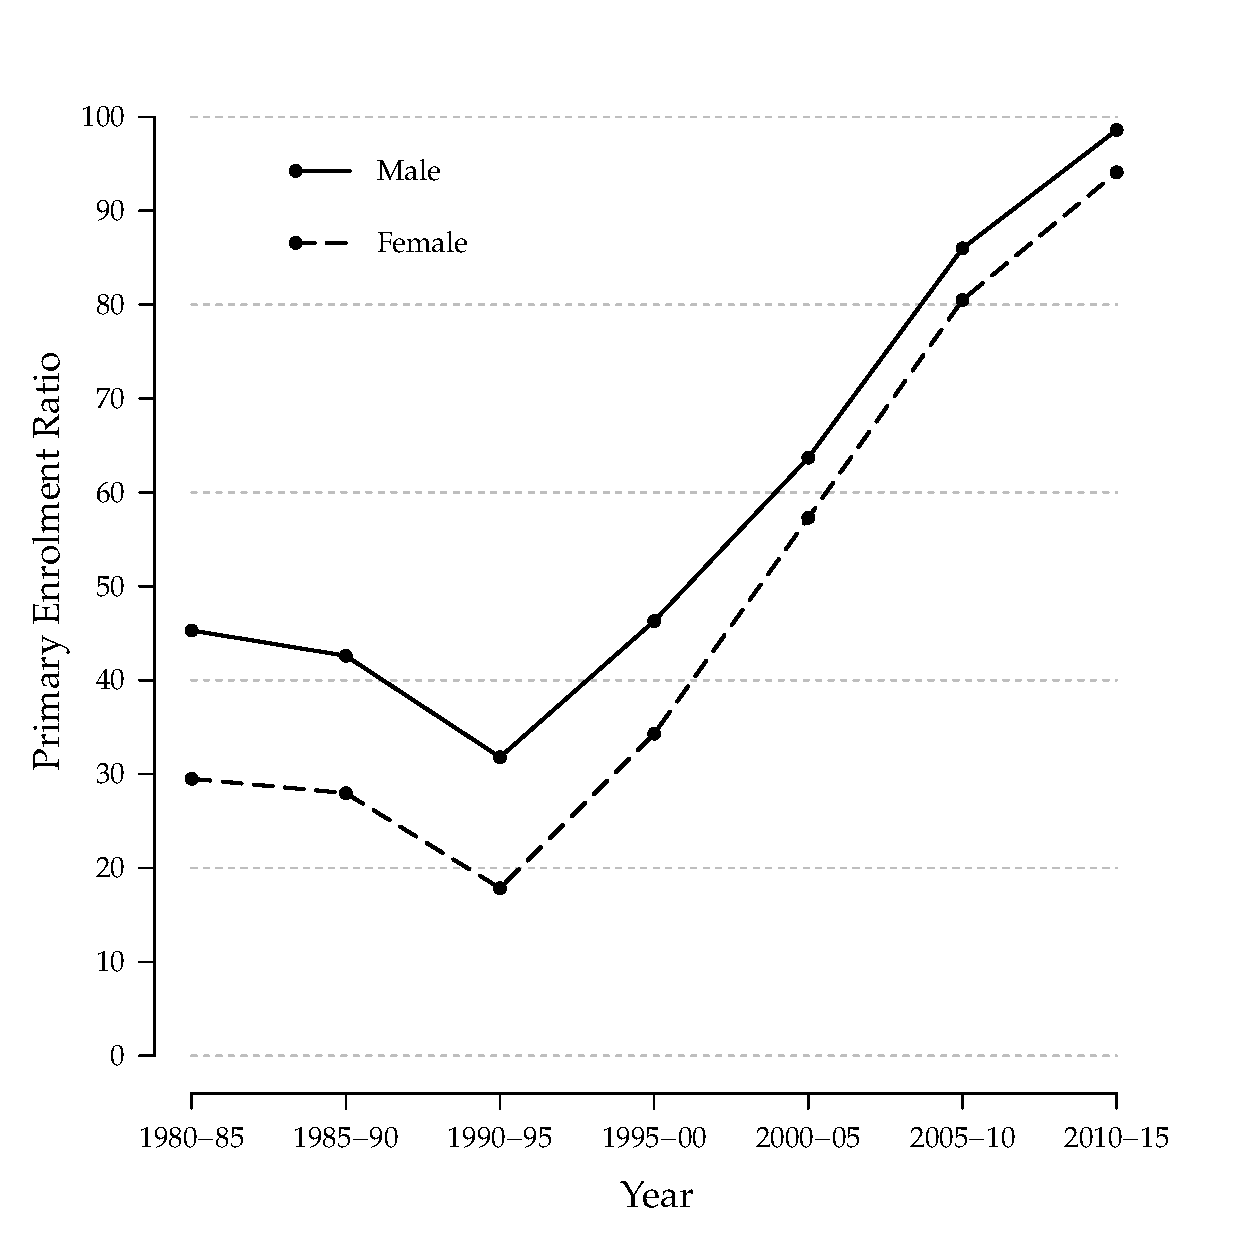
\includegraphics[width = \columnwidth]{../figures/fig6.eps}
\caption{Fig 6}
\end{figure}

\lipsum[1]

\begin{figure}[!hbtp]
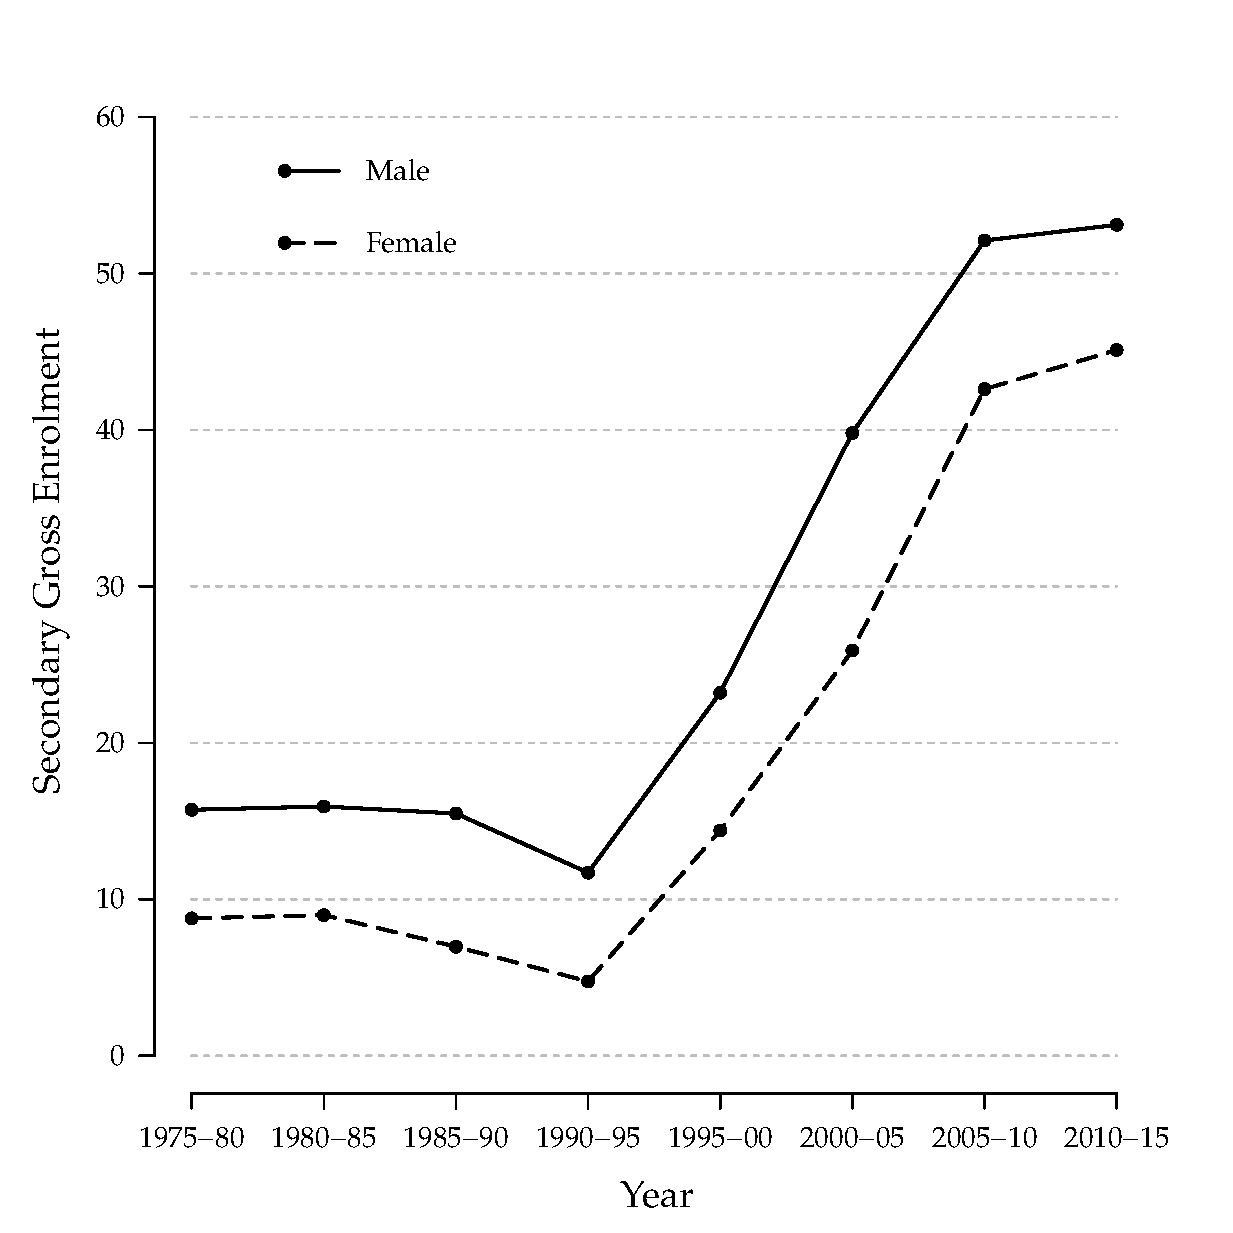
\includegraphics[width = \columnwidth]{../figures/fig7.eps}
\caption{Fig 7}
\end{figure}

\lipsum[1]


\end{document}
